\begin{sduDocument}
	\section{实验过程}
	\subsection{补全代码}
    \subsubsection{JavaScript}
    A sample JavaScript code snippet is shown below:
    \lstinputlisting[
        style = JavaScript,
        caption = {\bf Example of JavaScript},
        label = {lst:ExampleJs},
    ]{Code/Js/Example.js}
    
    \subsubsection{HTML}
    A sample HTML code snippet is shown below:
    \lstinputlisting[
        style = html,
        caption = {\bf Example of HTML},
        label = {lst:ExampleHtml},
    ]{Code/Html/Example.html}
    
    \subsubsection{CSS}
    A sample CSS code snippet is shown below:
    \lstinputlisting[
        style = css,
        caption = {\bf Example of CSS},
        label = {lst:ExampleCss},
    ]{Code/Css/Example.css}
    
    \subsection{Results Visualization}
    \begin{figure}[H]  % H option forces the figure to be placed exactly here
        \begin{subfigure}{0.45\textwidth}  % Left subfigure, width is 0.45 of text width
            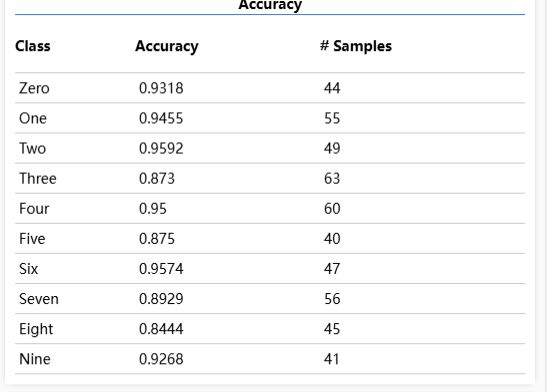
\includegraphics[width=\textwidth]{Figures/F1.jpg}  % Insert F1.jpg image
            \caption{\bf Accuracy}  % Subfigure caption
            \label{F1}  % Subfigure label for reference
        \end{subfigure}
        \hfill  % Horizontal fill space to separate the subfigures
        \begin{subfigure}{0.45\textwidth}  % Right subfigure, width is 0.45 of text width
            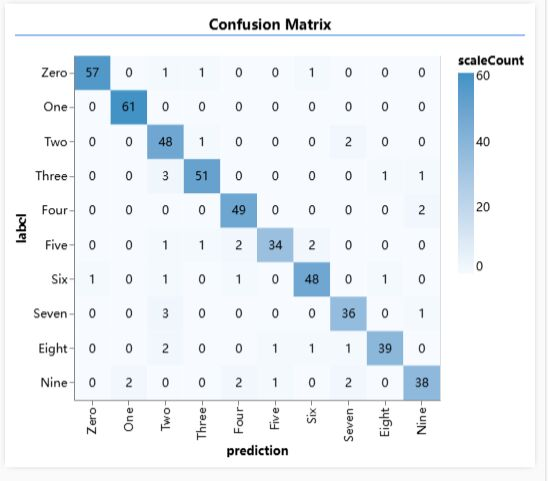
\includegraphics[width=\textwidth]{Figures/F2.jpg}  % Insert F2.jpg image
            \caption{\bf Confusion Matrix}  % Subfigure caption
            \label{F2}  % Subfigure label for reference
        \end{subfigure}
        \caption{Experimental Results}  % Main figure caption
        \label{fig:results}  % Main figure label for reference
    \end{figure}

    % Figure reference example
    The accuracy and confusion matrix results are shown in \cref{F1} and \cref{F2}. For comprehensive results, see \cref{fig:results2}.

    \begin{figure}[H]  % H option forces the figure to be placed exactly here
        \centering  % Center the figure
        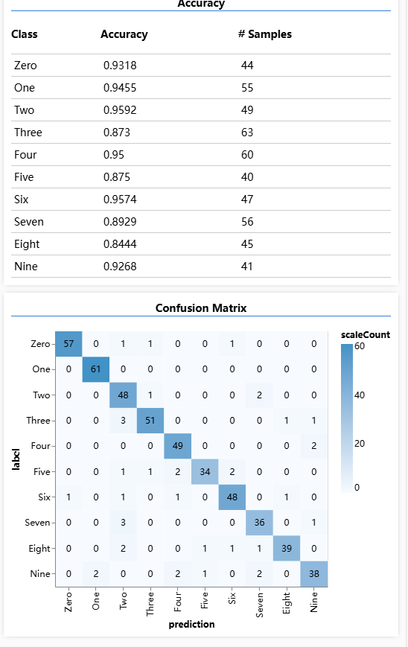
\includegraphics[width=0.5\textwidth]{Figures/F3.png}  % Insert F3.png image, width is 0.5 of text width
        \caption{\bf Comprehensive Experimental Results}  % Figure caption
        \label{fig:results2}  % Figure label for reference
    \end{figure}

    \section{实验心得与体会}  % Section for experimental reflections
\end{sduDocument}  % End of the document environment